\section{Auswertung}
\label{sec:Auswertung}

\subsection{Betimmung der Winkelrichtgröße}
Die Winkelrichtgröße wird aus Gleichung (7) bestimmt. In Tabelle (1) sind alle dafür benötigten Größen, also 
Abstand des Mittelpunktes der Drillachse zur angesetzten Federwaage, Auslenkungswinkel, und gemessene Kraft, dargestellt, 
wie zuletzt auch die berechnete Winkelrichtgröße. Dabei wurde für je einen Winkel zweimal der Abstand geändert und
gemessen. Die Unsicherheit des Abstandes wird auf 0.05 mm geschätzt.


\begin{table}[H]
  \centering
  \caption{Werte zur Berechnung der Winkelrichtgröße}
  \label{tab:Parameter}
  \begin{tabular}{c c c c}
    \toprule
    $\phi$/rad & $F/$N & r/m & $D/$Nm/$10^{-3}$\\
    \bottomrule
     0.52 & 0.46  & $0.02965 \pm 0.00005$ & $0.455 \pm 0.00077$ \\
     0.52 & 0.26  & $0.04945 \pm 0.00005$ & $0.429 \pm 0.00043$\\
     0.70 & 0.62  & $0.02965 \pm 0.00005$ & $0.460 \pm 0.00076$\\
     0.70 & 0.39  & $0.04945 \pm 0.00005$ & $0.482 \pm 0.00049$\\
     0.87 & 0.80  & $0.02965 \pm 0.00005$ & $0.474 \pm 0.00080$\\
     0.87 & 0.48  & $0.04945 \pm 0.00005$ & $0.475 \pm 0.00048$\\
     1.05 & 0.94  & $0.02965 \pm 0.00005$ & $0.465 \pm 0.00078$\\
     1.05 & 0.57  & $0.04945 \pm 0.00005$ & $0.470 \pm 0.00048$\\
     1.22 & 1.10  & $0.02965 \pm 0.00005$ & $0.466 \pm 0.00079$\\
     1.22 & 0.66  & $0.04945 \pm 0.00005$ & $0.466 \pm 0.00047$\\
    \bottomrule
  \end{tabular}
\end{table}

Der Mittelwert aller Winkelrichtgrößen beträgt:

\begin{equation}
  D = (0.464 \pm 0.0005)\cdot 10^{-3} \symup{Nm}
\end{equation}






\subsection{Bestimmung des Trägheitsmoments der Drillachse}
In folgender Tabelle wird die Schwingungsdauer T und der zugehörige Abstand a vom Mittelpunk der Drillachse bis 
zum Schwerpunkt der Gewichte dargestellt. Dabei wurde für einen Abstand 10 Schwingungen gemessen und das Ergebnis
durch 10 geteilt. Der Fehler der Messung wird auf 0.5 Sekunden geschätzt.


\begin{table}[H]
  \centering
  \caption{Gemessene Schwingungsdauern und Abstände}
  \label{tab:Gemessene Schwingungsdauern und Abstände}
  \begin{tabular}{c c}
    \toprule
    $a/$mm & $T/$s \\
    \midrule
     $60 \pm 0.05$ & $2.46 \pm 0.05$ \\ 
     $80 \pm 0.05$ & $2.79 \pm 0.05$ \\
    $100 \pm 0.05$ & $3.16 \pm 0.05$ \\
    $120 \pm 0.05$ & $3.54 \pm 0.05$ \\
    $140 \pm 0.05$ & $3.97 \pm 0.05$ \\
    $160 \pm 0.05$ & $4.40 \pm 0.05$ \\
    $180 \pm 0.05$ & $4.86 \pm 0.05$ \\
    $200 \pm 0.05$ & $5.28 \pm 0.05$ \\
    $220 \pm 0.05$ & $5.76 \pm 0.05$ \\
    $240 \pm 0.05$ & $6.24 \pm 0.05$ \\
    \bottomrule
  \end{tabular}
\end{table} 


Das Quadrat der Schwingungsdauer wird gegen das Quadrat des Abstandes aufgetragen, und mit linearer Regression wird das Trägheitsmoment
der Drillachse berechnet. 

\begin{figure}[H]
  \centering
  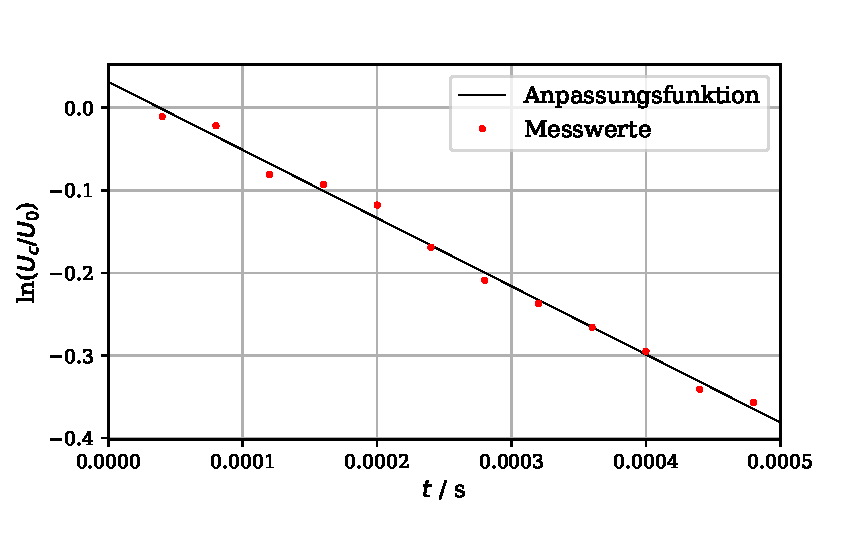
\includegraphics{plot1.pdf}
  \caption{Ausgleichsrechnung zur Bestimmung des Trägheitsmomentes der Drillachse.}
  \label{fig:plot}
\end{figure}

Beschrieben wird die Ausgleichsgerade durch folgende Gleichung:

\begin{equation}
  y = (592.91 \pm 11.52)x + (4.39 \pm 0.36)
\end{equation}

Mit Hilfe von Gleichung (5) ergibt sich:
\begin{align}
  T^2(a^2) = 4\pi^2\frac{(I_\text{D}+I_\text{K})}{D}
\end{align}
wobei $I_\text{K}$ das Trägheitsmoment der Gewichte ist, welches sich wie folgt zusammen setzt:

\begin{equation}
 I_\text{K} = (I_\text{Z1S}+I_\text{Z2S})+(m_\text{Z1}+m_\text{Z2})a^2
\end{equation}

$I_\text{Z1S}$ bzw. $I_\text{Z2S}$ sind die Trägheitsmomente der Zylinder-Gewichte mit Achse durch den Schwerpunkt.
Sie lassen sich mit der letzten Gleichung aus Abbildung (1) berechnen.
Die Masse der Gewichte beträgt:
\begin{equation}
m_\text{Z1} = 0.2218 kg , m_\text{Z2} = 0.2225 kg
\end{equation}
Der Durchmesser beider Gewichte beträgt $d = (0.03475 \pm 0.00005)m$ und die Höhe $h = (0.0297 \pm 0.00005)m$.
Die Werte für die Trägheitsmomente lauten also:
\begin{equation}
I_\text{Z1S} = (3.304 \pm 0.007)10^{-5} \symup{kgm^2}  , I_\text{Z2S} = (3.315 \pm 0.007)10^{-5} \symup{kgm^2} .
\end{equation}

Setzt man $I_\text{K}$ in Gleichung (11) ein, so ergibt sich:

\begin{equation}
 T^2(a^2) = 4\pi^2\frac{(I_\text{D}+(I_\text{Z1S}+I_\text{Z2S})+(m_\text{Z1}+m_\text{Z2})a^2)}{D}
\end{equation}
\begin{equation}
 \Rightarrow T^2(a^2) = \underbrace{4\pi^2\frac{(I_\text{D}+(I_\text{Z1S}+I_\text{Z2S}))}{D}}_{Achsenabschnitt \: b} + \underbrace{\frac{4\pi^2(m_\text{Z1}+m_\text{Z2})}{D}}_{Steigung \: m} a^2
 \end{equation}
 \begin{align}
  \Rightarrow I_D = \frac{bD}{4\pi^2}-(I_\text{ZS1}+I_\text{ZS2})
 \end{align}

 Das Trägheitsmoment der Drillachse beträgt:
 \begin{equation}
 I_D= (-1.5 \pm 0.4) \cdot 10^{-5} \symup{kgm^2} .
 \end{equation}


\subsection{Bestimmung des Trägheitsmoments für zwei Körper}
In diesem Auswertungsteil werden die Trägheitsmomente für eine Kugel und einen 
Zylinder berechnet, deren Drehachsen ihren Symmetrieachsen entsprechen.
Für die Kugel wurden je 8 Schwingungen gemessen, für den Zylinder je 5.
\begin{table}[H]
  \centering
  \caption{Schwingungsdauer eines Zylinder und einer Kugel}
  \label{tab:Schwingungsdauer von Zylinder und Kugel}
  \begin{tabular}{c c}
    \toprule
    $T_Z/$s & $T_K/$s \\
    \midrule
    $0.72 \pm 0.01$ & $1.47\pm 0.0625$ \\
    $0.75 \pm 0.01$ & $1.45\pm 0.0625$ \\
    $0.74 \pm 0.01$ & $1.48\pm 0.0625$ \\
    $0.74 \pm 0.01$ & $1.44\pm 0.0625$ \\
    $0.74 \pm 0.01$ & $1.46\pm 0.0625$ \\
  
    \bottomrule
  \end{tabular}
\end{table}

Als Mittelwerte ergeben sich:
\begin{equation}
T_Z = (0.74 \pm 0.04) s
\end{equation}
\begin{equation}
T_K = (0.146 \pm 0.028) s.
\end{equation}



Dadurch lassen sich mit Gleichung (8) die Trägheitsmomente berechnen:

\begin{equation}
I_Z = (6.4 \pm 0.8)\cdot 10^{-6} \symup{kgm^2}
\end{equation}
\begin{equation}
I_K = (2.51 \pm 0.1)\cdot 10^{-5} \symup{kgm^2} .
\end{equation}

Das negative Trägheitsmoment der Drillachse wurde bei der Berechnung nicht berücksichtigt,
da es physikalisch keinen Sinn ergibt. 
Berechnet man das Trägheitsmoment für einen Zylinder mit Masse $m = 0.3684 kg$, Durchmesser $d = (0.0973 \pm 0.00005) m$
und Höhe $h = (0.101 \pm 0.00005) m$ , ergibt sich: $I_Z =(4.36 \pm 0.004)10^{-4} \symup{kgm^2}$.
Der Theoriewert einer Kugel mit Masse $ m = 0.8123 kg$ und Durchmesser $ d = (0.13755 \pm 0.00005) m$
beträgt: $I_K = (1.54 \pm 0.001)10^{-3} \symup{kgm^2}$





\subsection{Bestimmung des Trägheitsmoments einer Modellpuppe}
\subsubsection{Berechnung über die gemessene Schwingungsdauer}
Es wird die Schwingungsdauer einer Puppe für zwei unterschiedliche 
Posen $P_\text{1}$ und $P_\text{2}$ bestimmt. Bei der ersten Pose sind Arme und Beine am Körper angewinkelt und in der zweiten
sind Arme senkrecht zum Körper nach außen gestreckt, und die Beine entgegengesetzt nach hinten bzw. vorne gestreckt.
Für die erste Pose werden 5 Schwingungen gemessen, für die zweite 10.
\begin{table}[H]
  \centering
  \caption{Schwingungsdauer der Modellpuppe}
  \label{tab:Schwingungsdauer der Modellpuppe}
  \begin{tabular}{c c}
    \toprule
    $T_{P_1}/$s & $T_{P_2}/$s \\
    \midrule
    $0.34 \pm 0.1$ & $0.85 \pm 0.05$ \\
    $0.35 \pm 0.1$ & $0.85 \pm 0.05$ \\
    $0.36 \pm 0.1$ & $0.84 \pm 0.05$ \\
    $0.38 \pm 0.1$ & $0.85 \pm 0.05$ \\
    $0.35 \pm 0.1$ & $0.86 \pm 0.05$ \\
    \bottomrule
  \end{tabular}
\end{table}

Als Mittelwerte ergeben sich:

\begin{equation}
T_{P_1} = (0.35 \pm 0.04) s
\end{equation}
\begin{equation}
T_{P_2}= (0.85 \pm 0.02) s
\end{equation}

Die Trägheitsmomente lassen sich analog zu den zwei Körpern mit Gleichung (8) berechnen.
Da Allerdings das Trägheitsmoment der Drillachse negativ ist, wird es in der Berechnung auf Null geschätzt:

\begin{equation}
I_{P_1}  = (1.5 \pm 0.4)\cdot 10^{-6} \symup{kgm^2} 
\end{equation}
\begin{equation}
I_{P_2}  = (8.5 \pm 0.4)\cdot 10^{-6} \symup{kgm^2} .
\end{equation}

\subsubsection{Berechnung über die Modellierung der Puppe}
Die Holzpuppe hat folgende Maße:\\
Kopf:\\
\begin{align*}
d_{\text{Kopf,Halbkugel}} &= (\num{30.9 +- 0.05})\,\si{\milli\meter}
\end{align*}
\begin{align*}
d_{\text{Kopf,1,Kegelstumpf}} &= (\num{30.9 +- 0.05})\,\si{\milli\meter} \\
d_{\text{Kopf,2,Kegelstumpf}} &= (\num{18.15 +- 0.05})\,\si{\milli\meter} \\
h_{\text{Kopf,Kegelstumpf}} &= (\num{35.4 +- 0.05})\,\si{\milli\meter} \\
d_{\text{Hals,Zylinder}} &= (\num{16 +- 0.05})\,\si{\milli\meter} \\
h_{\text{Hals,Zylinder}} &= (\num{10.7 +- 0.05})\,\si{\milli\meter}
\end{align*}
Oberkörper:\\
\begin{align*}
h_{\text{Oberkörper,1,Quader}} &= (\num{49.7 +- 0.05})\,\si{\milli\meter} \\
b_{\text{Oberkörper,1,Quader}} &= (\num{39.45 +- 0.05})\,\si{\milli\meter} \\
l_{\text{Oberkörper,1,Quader}} &= (\num{37 +- 0.05})\,\si{\milli\meter}
\end{align*}
\begin{align*}
d_{\text{Oberkörper,2,Zylinder}} &= (\num{24.9 +- 0.05})\,\si{\milli\meter} \\
h_{\text{Oberkörper,2,Zylinder}} &= (\num{15.15 +- 0.05})\,\si{\milli\meter}
\end{align*}
\begin{align*}
d_{\text{Oberkörper,3,Zylinder}} &= (\num{38.2 +- 0.05})\,\si{\milli\meter} \\
h_{\text{Oberkörper,3,Zylinder}} &= (\num{35.65 +- 0.05})\,\si{\milli\meter}
\end{align*}
Arm:\\
\begin{align*}
d_{\text{Arm,Kugel}} &= (\num{11.9 +- 0.05})\,\si{\milli\meter} \\
d_{\text{Arm,Zylinder}} &= (\num{12 +- 0.05})\,\si{\milli\meter} \\
h_{\text{Arm,Zylinder}} &= (\num{99.15 +- 0.05})\,\si{\milli\meter} \\
h_{\text{Hand,Quader}} &= (\num{24.7 +- 0.05})\,\si{\milli\meter} \\
b_{\text{Hand,Quader}} &= (\num{7.35 +- 0.05})\,\si{\milli\meter} \\
l_{\text{Hand,Quader}} &= (\num{12.9 +- 0.05})\,\si{\milli\meter}
\end{align*}
Bein:\\
\begin{align*}
d_{\text{Bein, Kugel}} &= (\num{12.05 +- 0.05})\,\si{\milli\meter} \\
d_{\text{Bein,1,Zylinder}} &= (\num{9.35 +- 0.05})\,\si{\milli\meter} \\
h_{\text{Bein,1,Zylinder}} &= (\num{56.8 +- 0.05})\,\si{\milli\meter} \\
d_{\text{Bein,2,Zylinder}} &= (\num{12.6 +- 0.05})\,\si{\milli\meter} \\
h_{\text{Bein,2,Zylinder}} &= (\num{6.9 +- 0.05})\,\si{\milli\meter} \\
d_{\text{Bein,3,Zylinder}} &= (\num{16.35 +- 0.05})\,\si{\milli\meter} \\
h_{\text{Bein,3,Zylinder}} &= (\num{61.35 +- 0.05})\,\si{\milli\meter} \\
h_{\text{Bein,Quader}} &= (\num{8.6 +- 0.05})\,\si{\milli\meter} \\
b_{\text{Bein,Quader}} &= (\num{15.45 +- 0.05})\,\si{\milli\meter} \\
l_{\text{Bein,Quader}} &= (\num{37.55 +- 0.05})\,\si{\milli\meter}.
\end{align*}
Für das Trägheitsmoment der Holzpuppe werden die Massen der einzelnen Körperteile benötigt.
Diese werden durch das Volumen der Bestandteile und das Gesamtgewicht bestimmt. Es wird angenommen,
dass eine homogene Massenverteilung vorliegt und dass die Arme und Beine paarweise identisch sind.
Das Volumen von Kugel, Kegelstumpf, Zylinder und Quader lassen sich durch
\begin{align*}
V_\text{K} &= \frac{4\pi}{3} \cdot R^3 &
V_\text{Ks} &= \frac{\pi h}{3} \cdot (R1^2 + R1 \cdot R2 + R2^2) \\
V_\text{Z} &= \pi \cdot R^2 \cdot h &
V_\text{Q} &= h \cdot b \cdot l
\end{align*}
und das Gesamtvolumen durch die Summe aller Einzelvolumina berechnen, wobei die der Arme und Beine
verdoppelt werden. Diese sind in Tabelle (5) zu finden.
\begin{table}[H]
\centering
\caption{Volumina der Körperteile und das Gesamtvolumen der Holzpuppe.}
\label{tab:puppe1}
\begin{tabular}{c c}
\toprule
Körperteil & $V \:/\: \cdot 10^{-5} \si{\cubic\meter}$ \\
\midrule
Kopf & $\num{2.697 +- 0.007}$ \\
Oberkörper & $\num{12.078 +- 0.002}$ \\
1 $\times$ Arm & $\num{1.444 +- 0.01}$ \\
1 $\times$ Bein & $\num{3.525 +- 0.012}$ \\
\midrule
\textit{Gesamt} & $\num{24.71 +- 0.04}$ \\
\bottomrule
\end{tabular}
\end{table}

Aus diesen ergibt sich mittels der Dichte 
\begin{align*}
\rho = \frac{Masse}{Volumen} = \frac{0.1626 \si{\kilo\gram}}{(\num{24.71 +- 0.04})\si{\cubic\meter}} = (\num{658 +- 1})\,\si{\kilo\gram\per\cubic\per\meter}
\end{align*}
die Massen der Körperteile, welche in Tabelle (6) zu finden sind.

\begin{table}[H]
\centering
\caption{Masse der Körperteile der Holzpuppe.}
\label{tab:puppemasse}
\begin{tabular}{c c c}
\toprule
Körperteil & $m \:/\: \si{\gram}$ \\
\midrule
Kopf & 17,75 \\
Oberkörper & 79,47 \\
1 $\times$ Arm & 9,50 \\
1 $\times$ Bein & 23,19 \\
\midrule
\textit{Gesamt} & 162,6 \\
\bottomrule
\end{tabular}
\end{table}

Die theoretischen Werte für das Trägheitsmoment werden mit dem Steiner'schen Satz und den Formeln aus
Abbildung (1) sowie
\begin{align*}
I_\text{Ks} = \frac{3}{10} m \frac{r_\text{2}^5 - r_\text{1}^5}{r_\text{1}^3 - r_\text{1}^3}
\end{align*}
bestimmt. Für das gesamte Trägheitsmoment der Figur in den Position $P_\text{1}$ und $P_\text{2}$ ergibt sich somit:
\begin{align*}
I_{\text{P}_1} &= (\num{4.09 +- 0.008})\cdot 10^{-5}\si{\kilo\gram\meter\squared} &
I_{\text{P}_2} &= (\num{53.14 +- 0.13})\cdot 10^{-5}\si{\kilo\gram\meter\squared}.
\end{align*}
